% This is "sig-alternate.tex" V2.0 May 2012
% This file should be compiled with V2.5 of "sig-alternate.cls" May 2012
%
% This example file demonstrates the use of the 'sig-alternate.cls'
% V2.5 LaTeX2e document class file. It is for those submitting
% articles to ACM Conference Proceedings WHO DO NOT WISH TO
% STRICTLY ADHERE TO THE SIGS (PUBS-BOARD-ENDORSED) STYLE.
% The 'sig-alternate.cls' file will produce a similar-looking,
% albeit, 'tighter' paper resulting in, invariably, fewer pages.
%
% ----------------------------------------------------------------------------------------------------------------
% This .tex file (and associated .cls V2.5) produces:
%       1) The Permission Statement
%       2) The Conference (location) Info information
%       3) The Copyright Line with ACM data
%       4) NO page numbers
%
% as against the acm_proc_article-sp.cls file which
% DOES NOT produce 1) thru' 3) above.
%
% Using 'sig-alternate.cls' you have control, however, from within
% the source .tex file, over both the CopyrightYear
% (defaulted to 200X) and the ACM Copyright Data
% (defaulted to X-XXXXX-XX-X/XX/XX).
% e.g.
% \CopyrightYear{2007} will cause 2007 to appear in the copyright line.
% \crdata{0-12345-67-8/90/12} will cause 0-12345-67-8/90/12 to appear in the copyright line.
%
% ---------------------------------------------------------------------------------------------------------------
% This .tex source is an example which *does* use
% the .bib file (from which the .bbl file % is produced).
% REMEMBER HOWEVER: After having produced the .bbl file,
% and prior to final submission, you *NEED* to 'insert'
% your .bbl file into your source .tex file so as to provide
% ONE 'self-contained' source file.
%
% ================= IF YOU HAVE QUESTIONS =======================
% Questions regarding the SIGS styles, SIGS policies and
% procedures, Conferences etc. should be sent to
% Adrienne Griscti (griscti@acm.org)
%
% Technical questions _only_ to
% Gerald Murray (murray@hq.acm.org)
% ===============================================================
%
% For tracking purposes - this is V2.0 - May 2012

\documentclass{sig-alternate}

%% customization goes into input macros
% set up tight list spacing
\usepackage{enumitem} 
\setlist{nolistsep,nosep}

% for toggles
\usepackage{etoolbox}

\newcommand {\studyquote}[1]{\em ``#1''\normalfont}

% CHANGE FROM TOGGLE TRUE TO TOGGLE FALSE FOR NON-ANONYMOUS RENDERING
% http://tex.stackexchange.com/questions/5894/latex-conditional-expression
\newtoggle{anonymous}
%\toggletrue{anonymous}
\togglefalse{anonymous}

% CHANGE FROM TOGGLE TRUE TO TOGGLE FALSE TO HIDE COMMENTS
\newtoggle{comments}
%\toggletrue{comments}
\togglefalse{comments}

% Comment region command (from Wesley Willett)
\usepackage[usenames]{color}
\usepackage[usenames,dvipsnames]{xcolor}
\iftoggle{comments} {
  %if we want to show comments
  %% ============================================================
  %% add your names here
  %% possible colors include:
  %%   Orange, magenta, NavyBlue, violet, BrickRed, OliveGreen
  %% ============================================================
  \newcommand {\ben}[1]{{\color{BrickRed}\bf{BZ: #1}\normalfont}}
  \newcommand {\yuxun}[1]{{\color{OliveGreen}\bf{YX: #1}\normalfont}}
}{
  %if we don't want to show comments
  \newcommand {\ben}[1]{}
  \newcommand {\yuxun}[1]{}
}

% \newcommand {\systemname}{HOBS }
% \newcommand {\systemnamenospace}{HOBS}


%%% Local Variables: 
%%% mode: latex
%%% TeX-master: "main"
%%% End: 



\begin{document}
%
% --- Author Metadata here ---
%\conferenceinfo{WOODSTOCK}{'97 El Paso, Texas USA}
%\CopyrightYear{2007} % Allows default copyright year (20XX) to be over-ridden - IF NEED BE.
%\crdata{0-12345-67-8/90/01}  % Allows default copyright data (0-89791-88-6/97/05) to be over-ridden - IF NEED BE.
% --- End of Author Metadata ---

\title{Which Device Knows Your Activity Better,\\ Google Glass, Mobile Phones or Pebble Smartwatch?}
% \subtitle{[Extended Abstract]
% \titlenote{A full version of this paper is available as
% \textit{Author's Guide to Preparing ACM SIG Proceedings Using
% \LaTeX$2_\epsilon$\ and BibTeX} at
% \texttt{www.acm.org/eaddress.htm}}}
%
% You need the command \numberofauthors to handle the 'placement
% and alignment' of the authors beneath the title.
%
% For aesthetic reasons, we recommend 'three authors at a time'
% i.e. three 'name/affiliation blocks' be placed beneath the title.
%
% NOTE: You are NOT restricted in how many 'rows' of
% "name/affiliations" may appear. We just ask that you restrict
% the number of 'columns' to three.
%
% Because of the available 'opening page real-estate'
% we ask you to refrain from putting more than six authors
% (two rows with three columns) beneath the article title.
% More than six makes the first-page appear very cluttered indeed.
%
% Use the \alignauthor commands to handle the names
% and affiliations for an 'aesthetic maximum' of six authors.
% Add names, affiliations, addresses for
% the seventh etc. author(s) as the argument for the
% \additionalauthors command.
% These 'additional authors' will be output/set for you
% without further effort on your part as the last section in
% the body of your article BEFORE References or any Appendices.

\numberofauthors{2} %  in this sample file, there are a *total*
% of EIGHT authors. SIX appear on the 'first-page' (for formatting
% reasons) and the remaining two appear in the \additionalauthors section.
%

\iftoggle{anonymous}{
  \author{
    \alignauthor 
    Anonymous for submission
  }
}{ %else
  \author{
    % You can go ahead and credit any number of authors here,
    % e.g. one 'row of three' or two rows (consisting of one row of three
    % and a second row of one, two or three).
    % 
    % The command \alignauthor (no curly braces needed) should
    % precede each author name, affiliation/snail-mail address and
    % e-mail address. Additionally, tag each line of
    % affiliation/address with \affaddr, and tag the
    % e-mail address with \email.
    \alignauthor Ben Zhang \\
    \affaddr{UC Berkeley EECS}\\
    \email{benzh@eecs.berkeley.edu}
    % 2nd. author
    \alignauthor Yuxun Zhou \\
    \affaddr{UC Berkeley EECS} \\
    \email{yxzhou@eecs.berkeley.edu}
  }
}

\maketitle
\begin{abstract}
We believe that for activity recognition tasks, different devices will have different performance. However, it's unclear that 1) which device is better for which activity, 2) the quantitative differnece. In this project, we compare the activity recognition accuracy for two devices -- Google Glass and android phones. Through our extensive studies, we have found that Glass is better than phones in general, and with the same algorithm, Glass outperforms phone by XX\%.
\end{abstract}

% A category with the (minimum) three required fields
% \category{H.4}{Information Systems Applications}{Miscellaneous}
%A category including the fourth, optional field follows...
% \category{D.2.8}{Software Engineering}{Metrics}[complexity measures, performance measures]

% \terms{Theory}

\keywords{Activity Recognition; Google Glass; Android Phones; HMM}

%% The outline comes from this link: http://www.cosc.canterbury.ac.nz/open/students/peyton-jones-writing_a_paper-slides.pdf
\section{Introduction}
\label{sec:introduction}

Introduction usually contains two parts:
\begin{itemize}
\item Describe the problem. Using examples are recommended.
\item State your contributions. Bulleted list of contributions. Contributions should be refutable.
\end{itemize}


%%% Local Variables: 
%%% mode: latex
%%% TeX-master: "main"
%%% End: 


\section{Problem Formulation}
\label{sec:problem-formulation}

A supervised learning framework for activity recognition consist of data collection, transformation, and the design of adequate learning algorithm. In this section, we first briefly describe our data collection protocol, and detailed system description is postponed to section (\ref{sec:awesome-system}) for completeness. In section (\ref{subsec: data-transform}), we show how raw data is transformed into feature space. In addition, the problem of feature selection  for efficient learning is discussed. In Section (\ref{subsec: learning}), we formulate the learning problem, and propose two methods for a comparative study.  

\subsection{Data Collection}
\label{subsec: data-collection}
In order to collect varies sensor data from devices such as Android phones and Google glass, an awesome system is designed and deployed which pulls readings of accelerometers, gyroscope, magnetic and gravity sensor continuously into a database. Section (\ref{sec:awesome-system}) is devoted for more details of this setup. From a data analysis point of view, the obtained observations are a set of time series of sensor readings with descent time resolution of up to 10 nano seconds, and the labels are corresponding five factors $[1 to 5]$ each representing a specific activity.

The data is collected in a controlled manner, i.e. we asked one experimenter wearing all devices to perform activities as requested, and anther experimenter served as supervisor recording starting/ending time of each activity in the sequence. Hence labels of the a sample could be found easily by looking at the time slot. Note that IRB is a necessity for this kind of experiment if more volunteers are involved, thus for now the experiment is only conducted by two people(the two authors...) 

\subsection{Data Transformation and Feature Selection}
\label{subsec: data-transform}


\subsection{Activity Recognition as Supervised Learning}
\label{subsec: learning}

Concentrate single-mindedly on a narrative that:
\begin{itemize}
\item Describes the problem, and why it is interesting
\item Describes your idea
\item Defends your idea, showing how it solves the problem, and filling out the details.
\end{itemize}
On the way, cite relevant work in passing, but defer discussion to the end

%%% Local Variables: 
%%% mode: latex
%%% TeX-master: "main"
%%% End: 

\section{System and Data}
\label{sec:data-collection}

In this section, we describe our system -- Android platform and Pebble platform. We then briefly cover the experiement setup. \ben{maybe this should be in introduction.} Throughout the paper, we use {\em Phone} for mobile phones, and {\em Glass}, {\em Pebble} for Google Glass and Pebble Smartwatch, respetively.


\subsection{Android Platform}
\label{sec:android-platform}

Our Android application is adapted from BearLoc\footnote{BearLoc is developed by Software Defined Buildings (SDB) group at Berkeley; the intial goal of that project is to provide an open-source implementation that is targeted at indoor semantic localization service.}. We built a continous sensor monitoring application on top of \texttt{BearLocService} which makes sensor data collection

Our initial application involves sampling all sorts of sensor data from Android platform, including acclerometer, gyroscope, magnetic field, light, GPS, WiFi signals, etc. However, through some preliminary study, we have found that mobile phones and Google Glass cannot easily handle the extensive sensing tasks, especially when we are trying to sample acceleration in a relative high frequency. Since we are interested in the comparison among these wearable devices and Pebble only has a 3D accelerometer, we implemented our Android application only for sampling acclerometer data.

The sensor data is obtained through \texttt{onSensorChanged()} API provided by Android OS. The sampling frequency is resource adaptive -- it turns out to be 100Hz for phones and 50Hz for Glass. 

Once the data is measured, we record the time in millisecond accuracy by calling \texttt{System.currentTimeMillis()}. To extract the data, we logged the data locally by writing to a \texttt{csv} file and also post a HTTP request that saves the data to \texttt{MongoDB}.

\subsection{Pebble Platform}
\label{sec:pebble-platform}

The Pebble accelerometer data collection application is based on \texttt{AccelerometerService} API provided by Pebble OS. We register a callback function as the handler whenever accelerometer data is available. The callback function operates on \texttt{AccelData} which already has a field of timestamp in millisecond accuracy. 

The data storage and transmission is supported by \texttt{DataLogging} API which requires a customized Android application that uses Pebble SDK to retrieve logs by application universally unique identifier (UUID). We have also developed this accompany Android application for retrieving the data and writing them into a \texttt{csv} file for data analysis.

\subsection{Accelerometer Data}
\label{sec:accelerometer-axes}

On both Android and Pebble platform, the acclerometer coordinate system is defined relative to the device's screen (see Figure~\ref{fig:coordinate}). When the user is facing the screen, the axes are:
\begin{itemize}
\item x: horizontal and points to the right.
\item y: vertical and points up.
\item z: points towards the outside of of the screen face.
\end{itemize}

 
%% 04-20 17:40:46.392    4187-4187/name.benzhang.hellostep.app I/HelloStep﹕ {Sensor name="MPL Accelerometer", vendor="Invensense", version=1, type=1, maxRange=19.6133, resolution=0.039226603, power=0.0, minDelay=1000}

%% { "_id" : ObjectId("536f303fe0323929bee2cf88"), "vendor" : "STMicroelectronics", "power" : 0.23000000417232513, "min delay" : 20000, "resolution" : 0.01362034771591425, "sysnano" : NumberLong("170075408653778"), "epoch" : NumberLong("1399795756898"), "version" : 1, "max range" : 19.613300323486328, "type" : "sensor info", "model" : "KR3DM 3-axis Accelerometer", "sensor" : "accelerometer", "id" : "9026086e-bd07-3f96-9622-757da2907a93" }

However, the data differs in range, resolution and sample frequency. We use $g$ to denote the gravitational accelerometer constant (normal $9.81 m/s^2$). In Table~\ref{tab:sensorinfo}, we have listed the sensor information. Note that in our project, we have been using Samsung Galaxy S II, so the information is for that particular device. 

\begin{table}
  \centering
  \begin{tabular}{c|c|c|c}
    \hline
    Device & max range & resolution & sample frequency \\
    \hline
    Phone  & 19.6g     & 0.013g     & 100Hz  \\
    Glass  & 19.6g     & 0.039g     & 50Hz   \\
    Pebble & 4g        & 0.008g     & 25Hz   \\
    \hline
  \end{tabular}
  \label{tab:sensorinfo}
  \caption{Sensor information of the devices.}
\end{table}

\begin{figure}
  \centering
  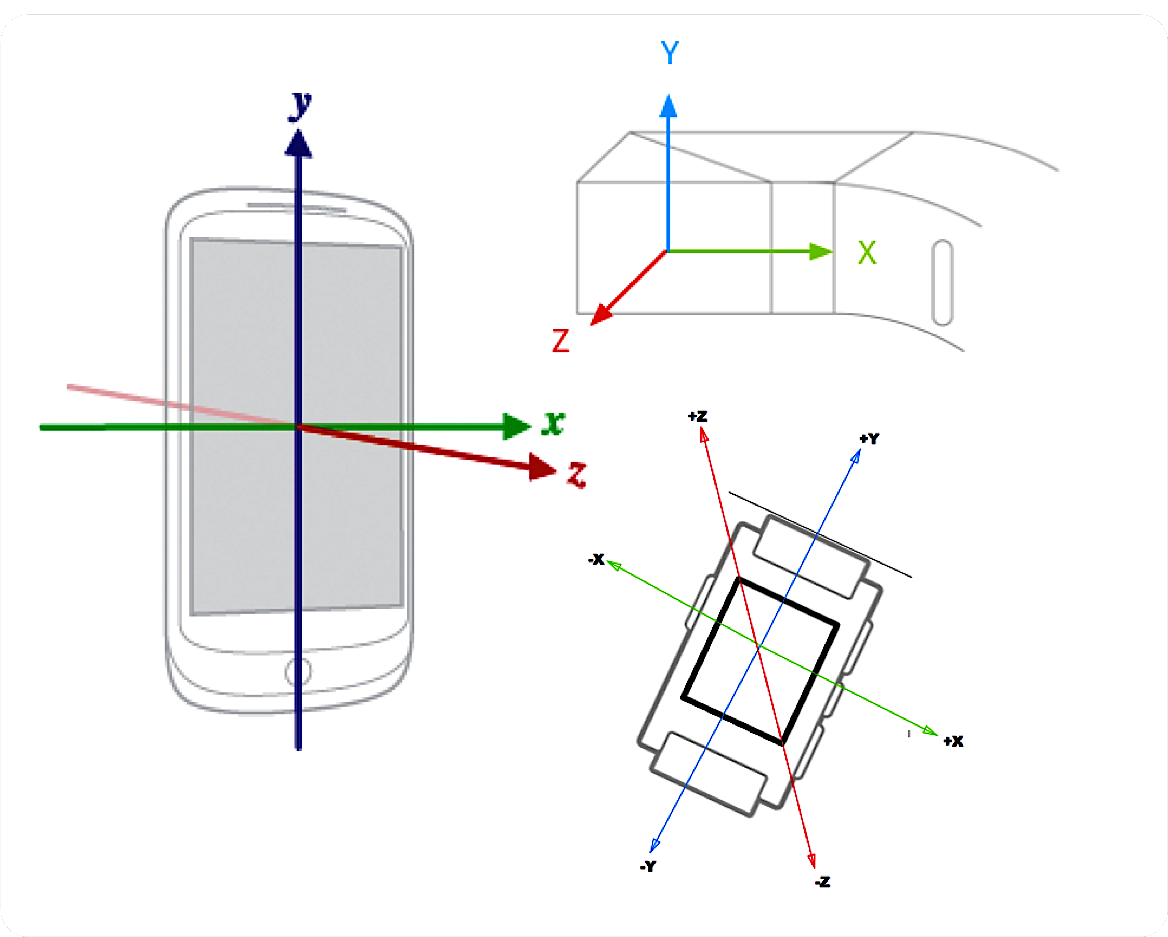
\includegraphics[width=0.9\columnwidth]{figures/coordinates.png}
  \caption{3D co-ordinate system of our hardware platforms.}
  \label{fig:coordinate}
\end{figure}

\subsection{Data Collection}
\label{sec:data-collection-2}

With our data collection platform, we have performed a series of activities and collected the acclerometer data. Figure~\ref{fig:exp} shows how these devices are worn on a user and the experiement is being conducted. To obtain the ground truth, we use an extra iPhone to take videos continuously during the study. The video is manually processed to label the collected acclerometer data.

\begin{figure}
  \centering
  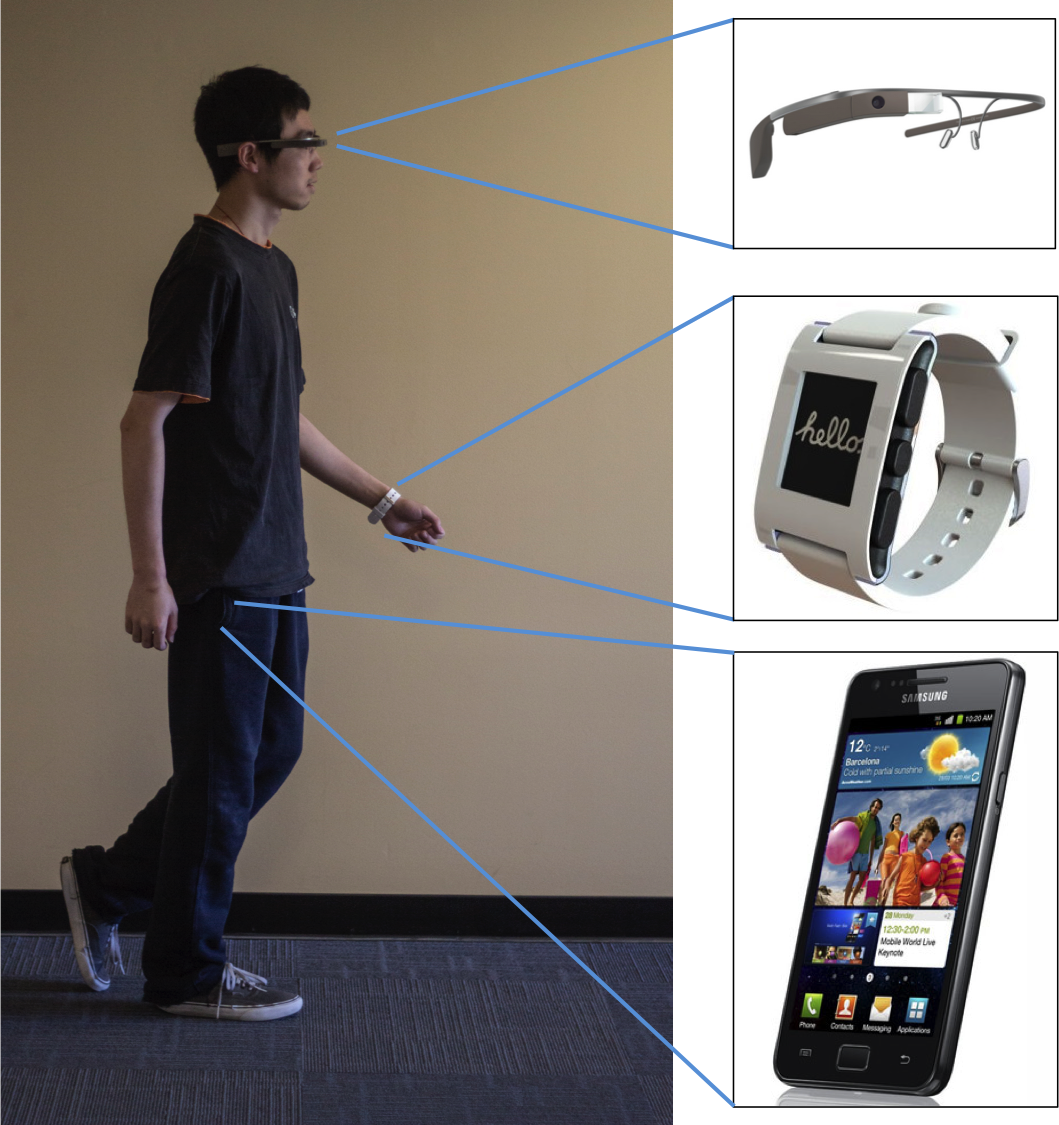
\includegraphics[width=0.9\columnwidth]{figures/experiement_setup.png}
  \caption{Data collection process of simutaneously wearing three different devices and an illustration of their relative positions on the testee's body.}
  \label{fig:exp}
\end{figure}



%%% Local Variables: 
%%% mode: latex
%%% TeX-master: "main"
%%% End: 


\section{Evaluation}
\label{sec:evaluation}

In this section, we present our data and the results of our algorithm.

\subsection{Raw Data and Extracted Features: EDA}
The raw data sets are shown in Figure~\ref{fig:soda1} and \ref{fig:soda2} with ground truth labels. A quick glance tell us that the three devices we are using generate measurement of different quality as far as classification is concerned. For example, in all axis $\{x,y,z\}$, Phone yields measurement with little noise. 

\begin{figure*}
  \centering
  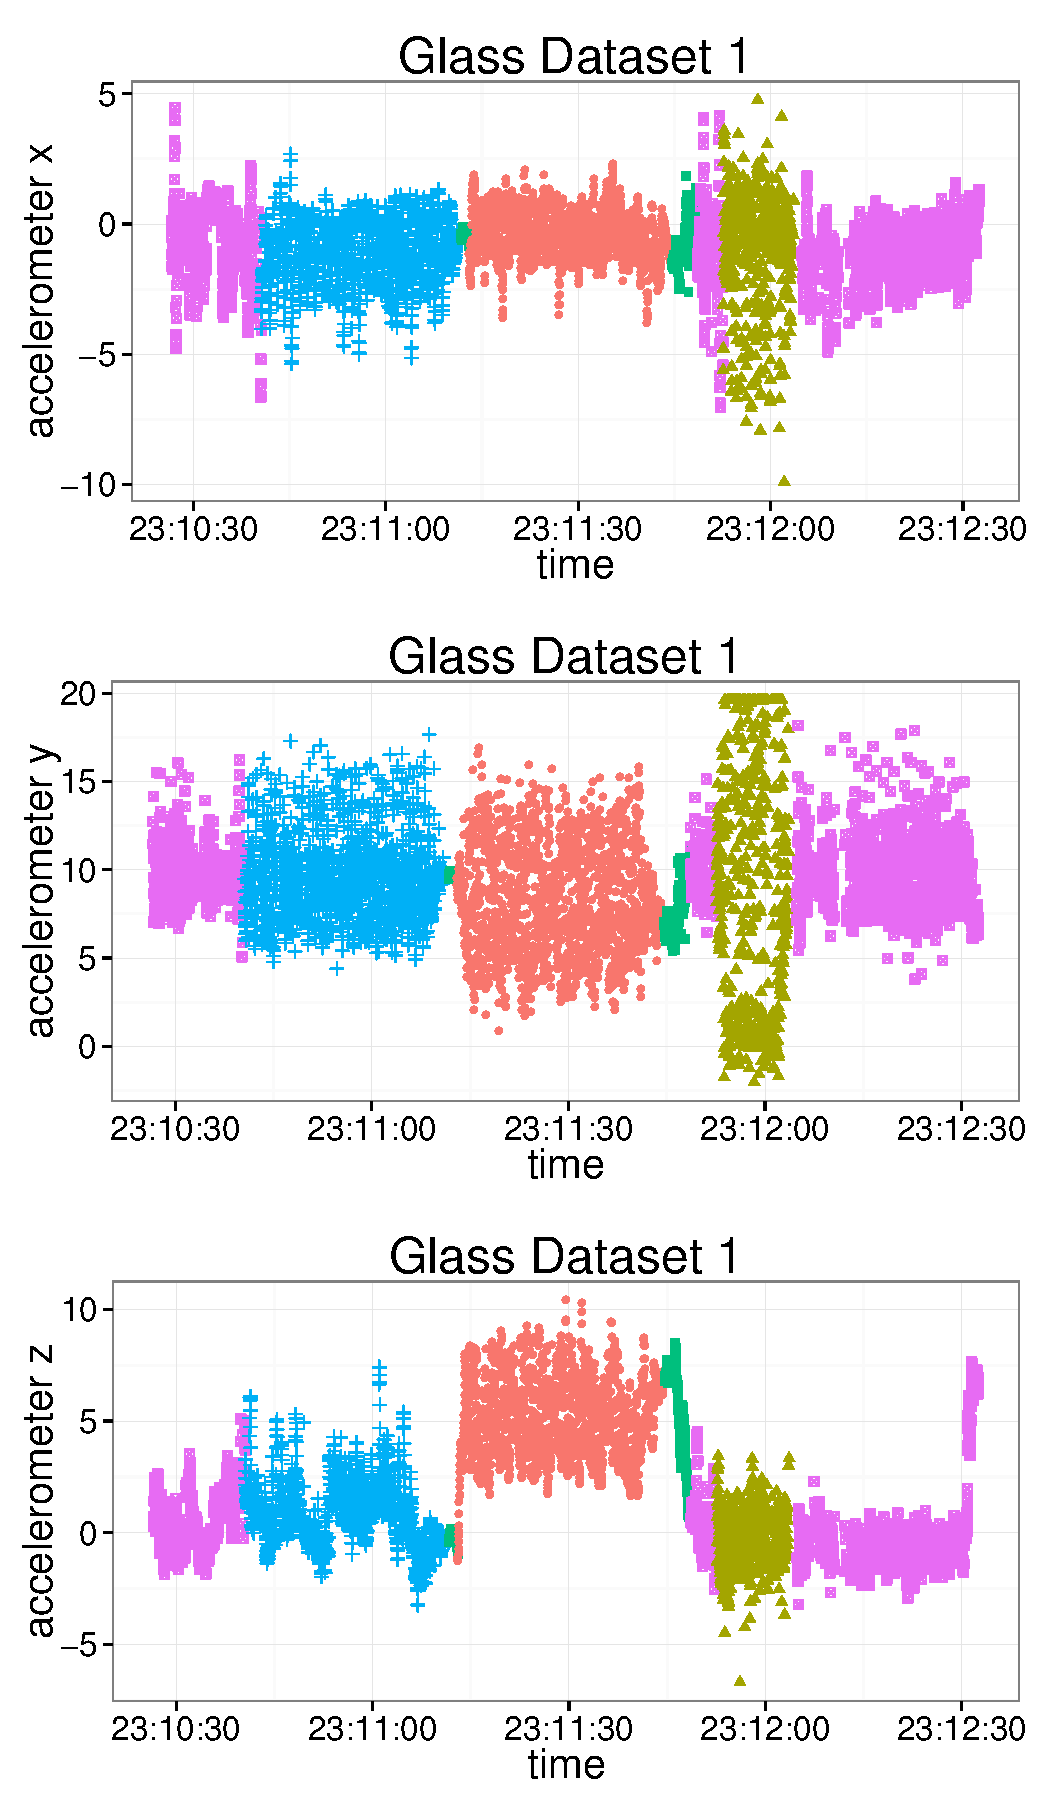
\includegraphics[width=0.3\textwidth]{figures/eda_soda1_glass.pdf}
  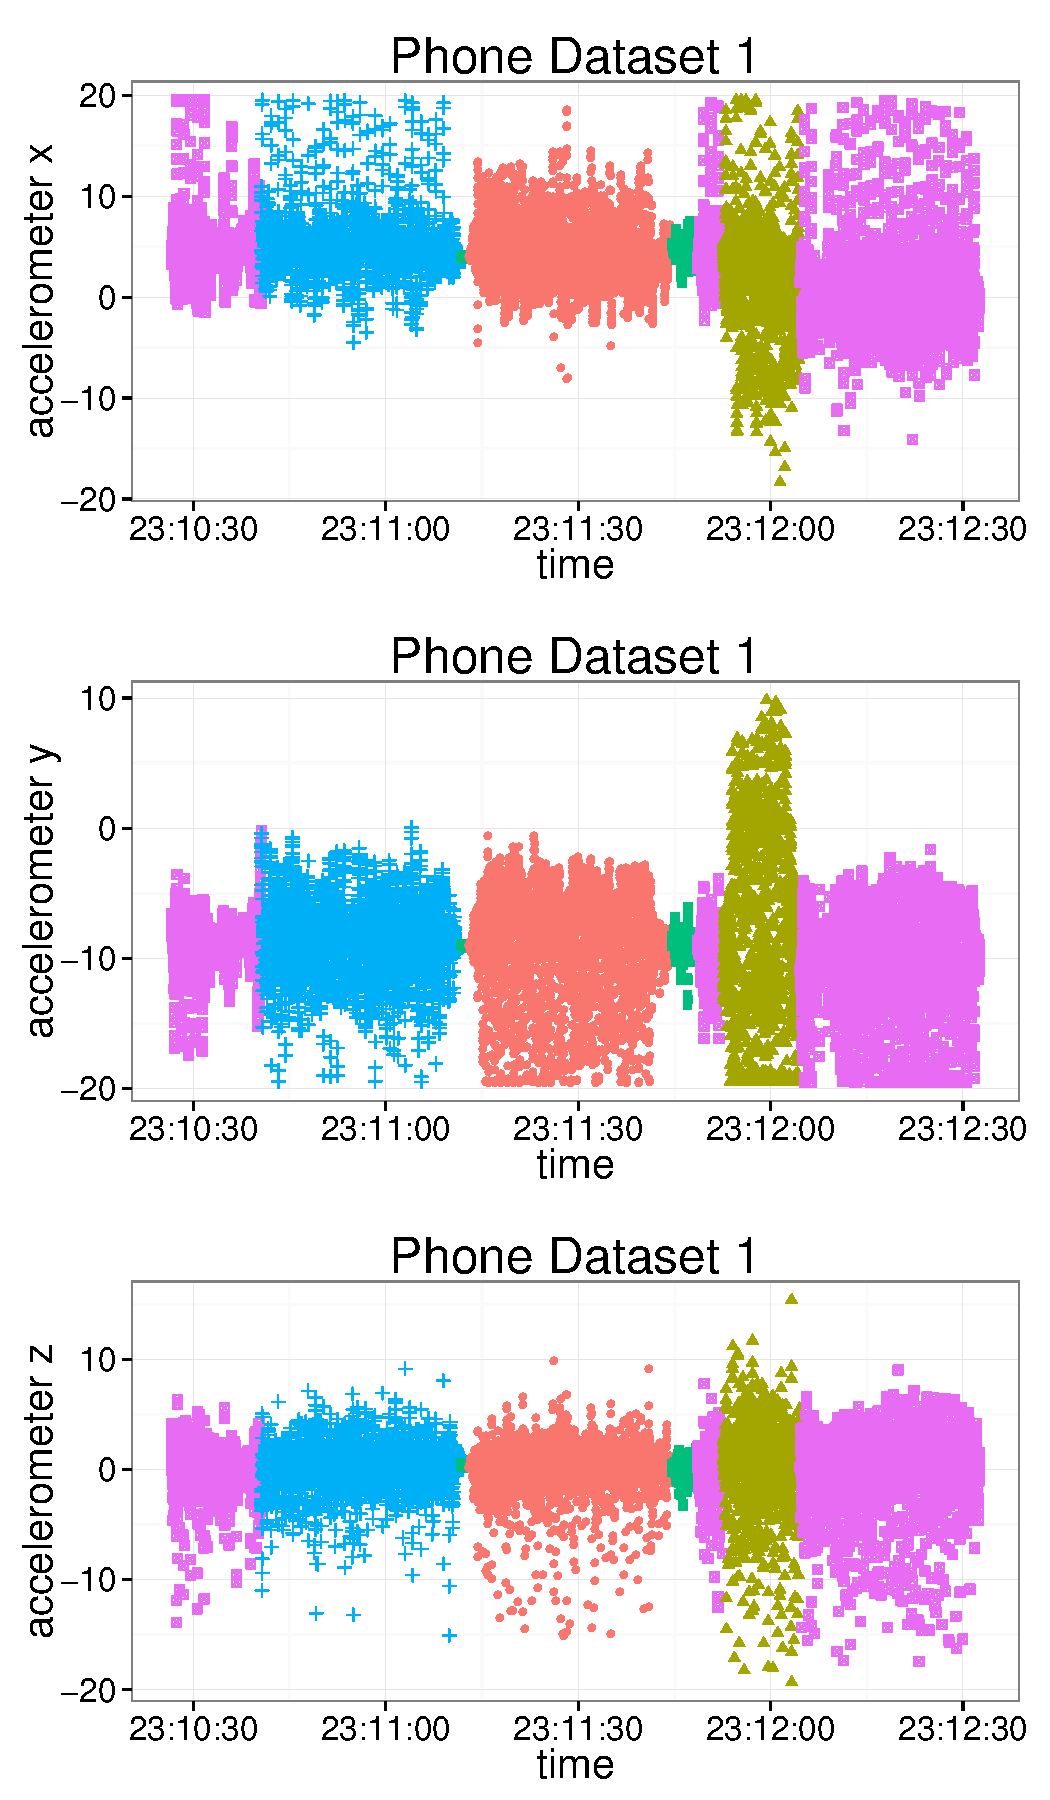
\includegraphics[width=0.3\textwidth]{figures/eda_soda1_phone.pdf}
  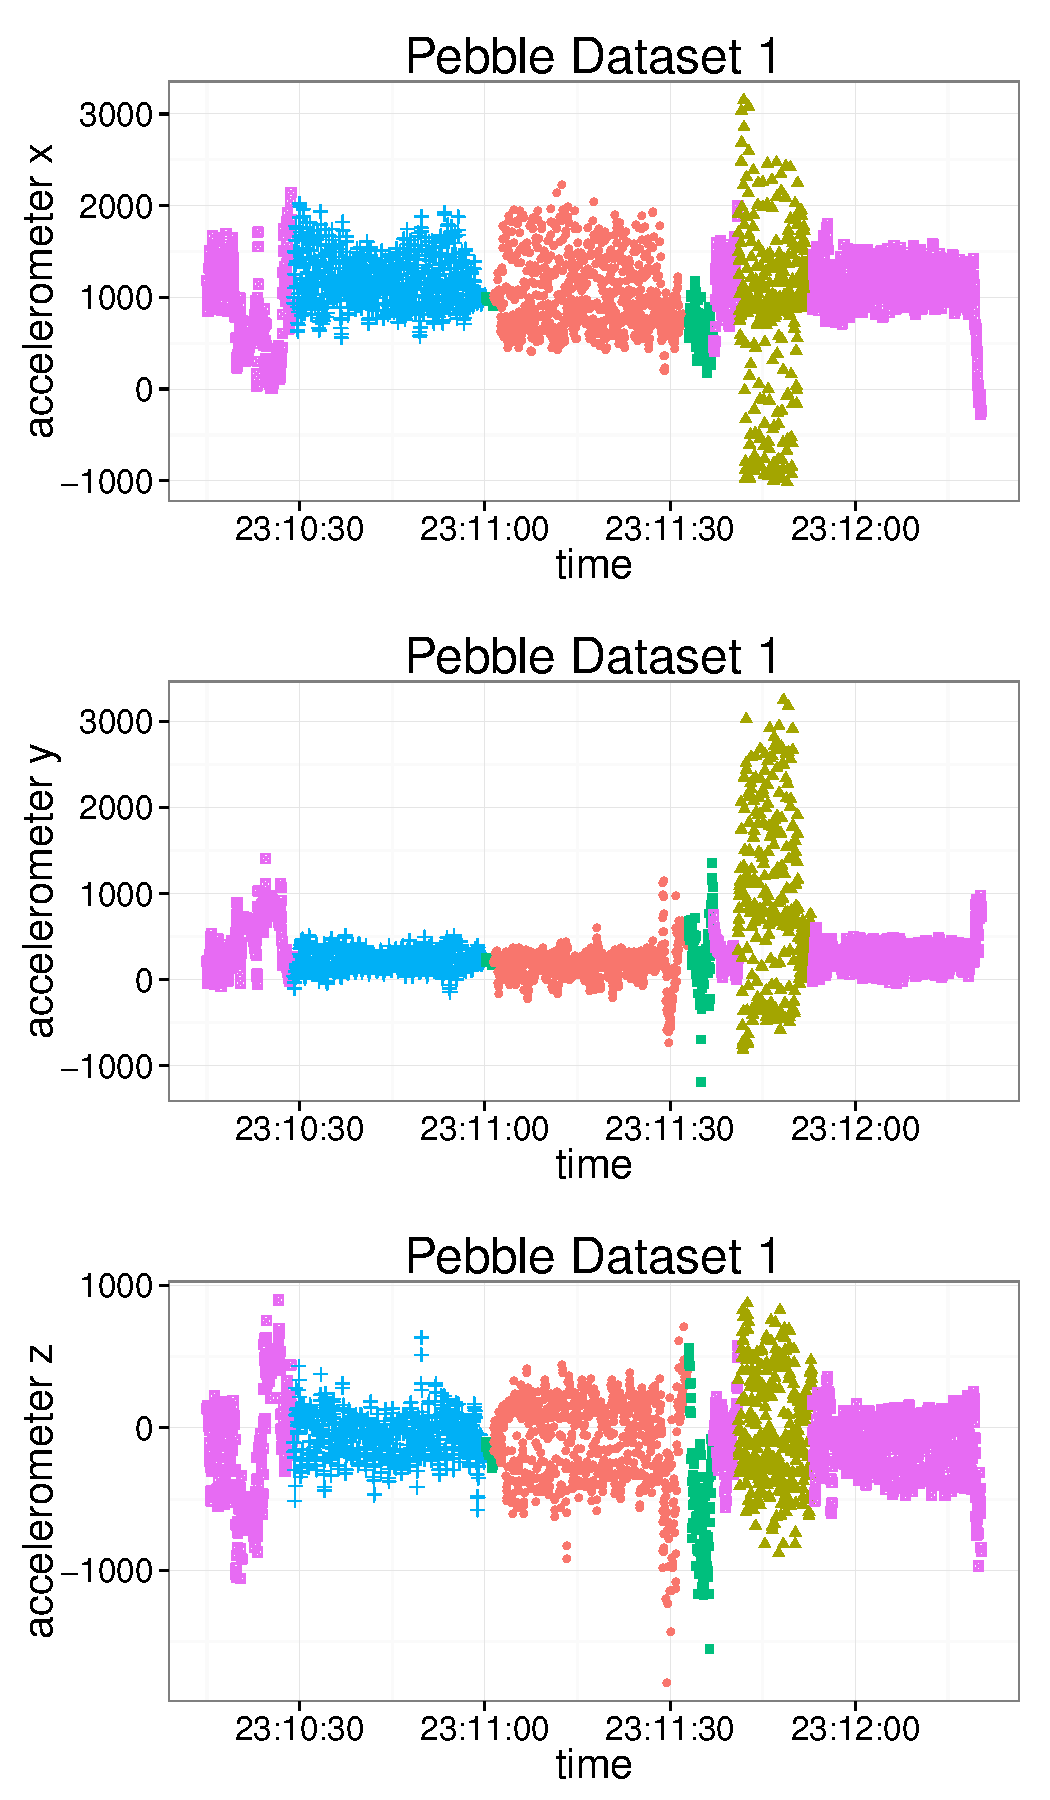
\includegraphics[width=0.3\textwidth]{figures/eda_soda1_pebble.pdf}
  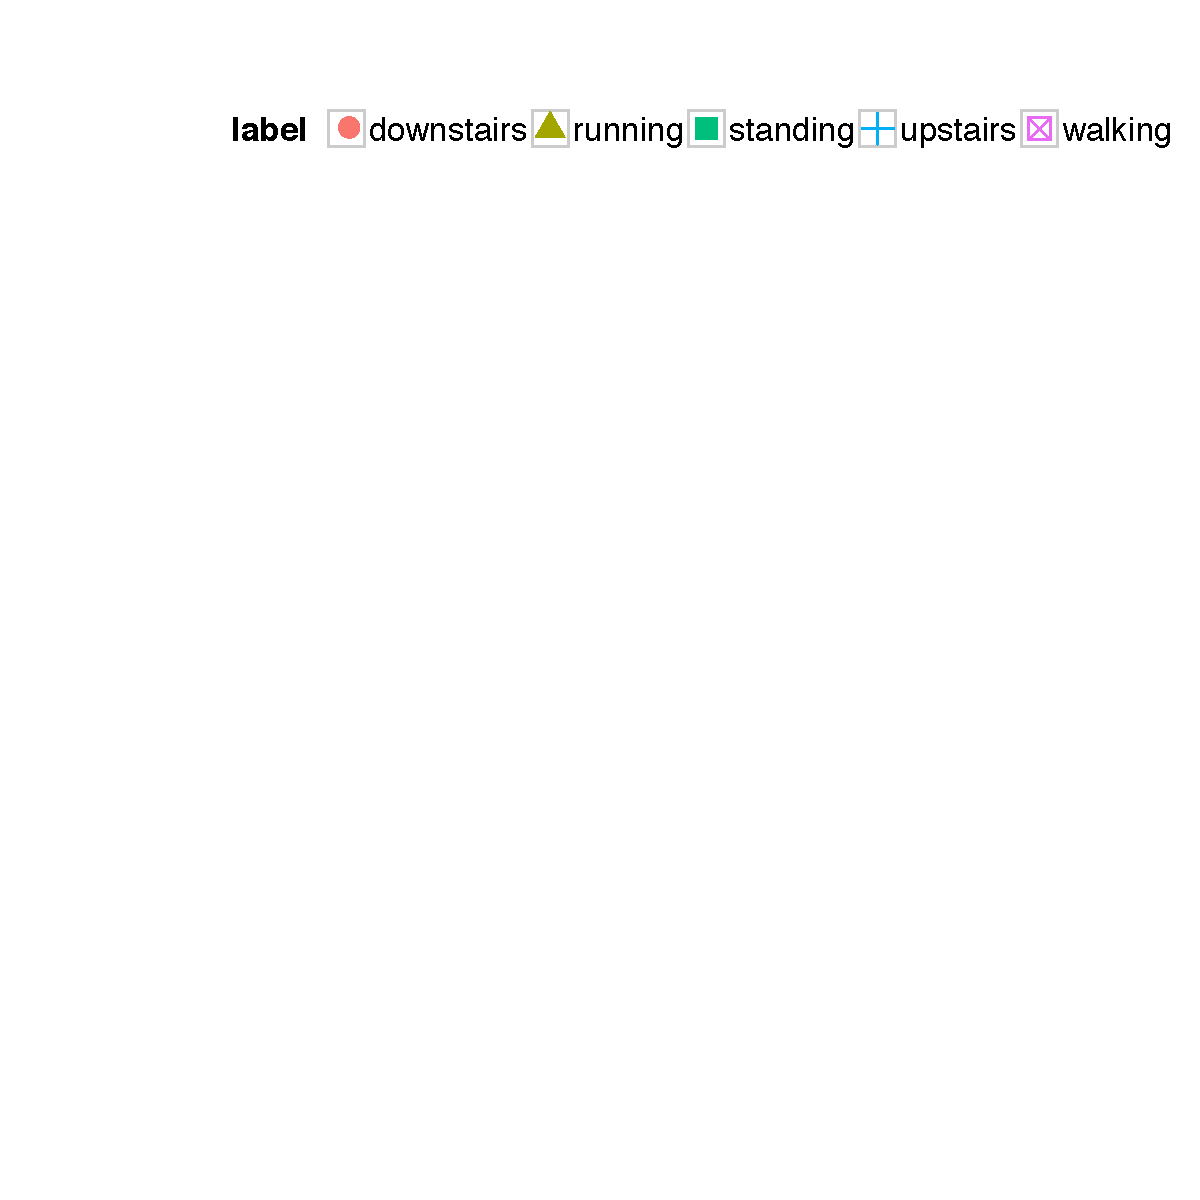
\includegraphics[width=0.5\textwidth]{figures/legend.pdf}
  \caption{The first raw data set visualization with groundtruth labeled.}
  \label{fig:soda1}
\end{figure*}

\begin{figure*}
  \centering
  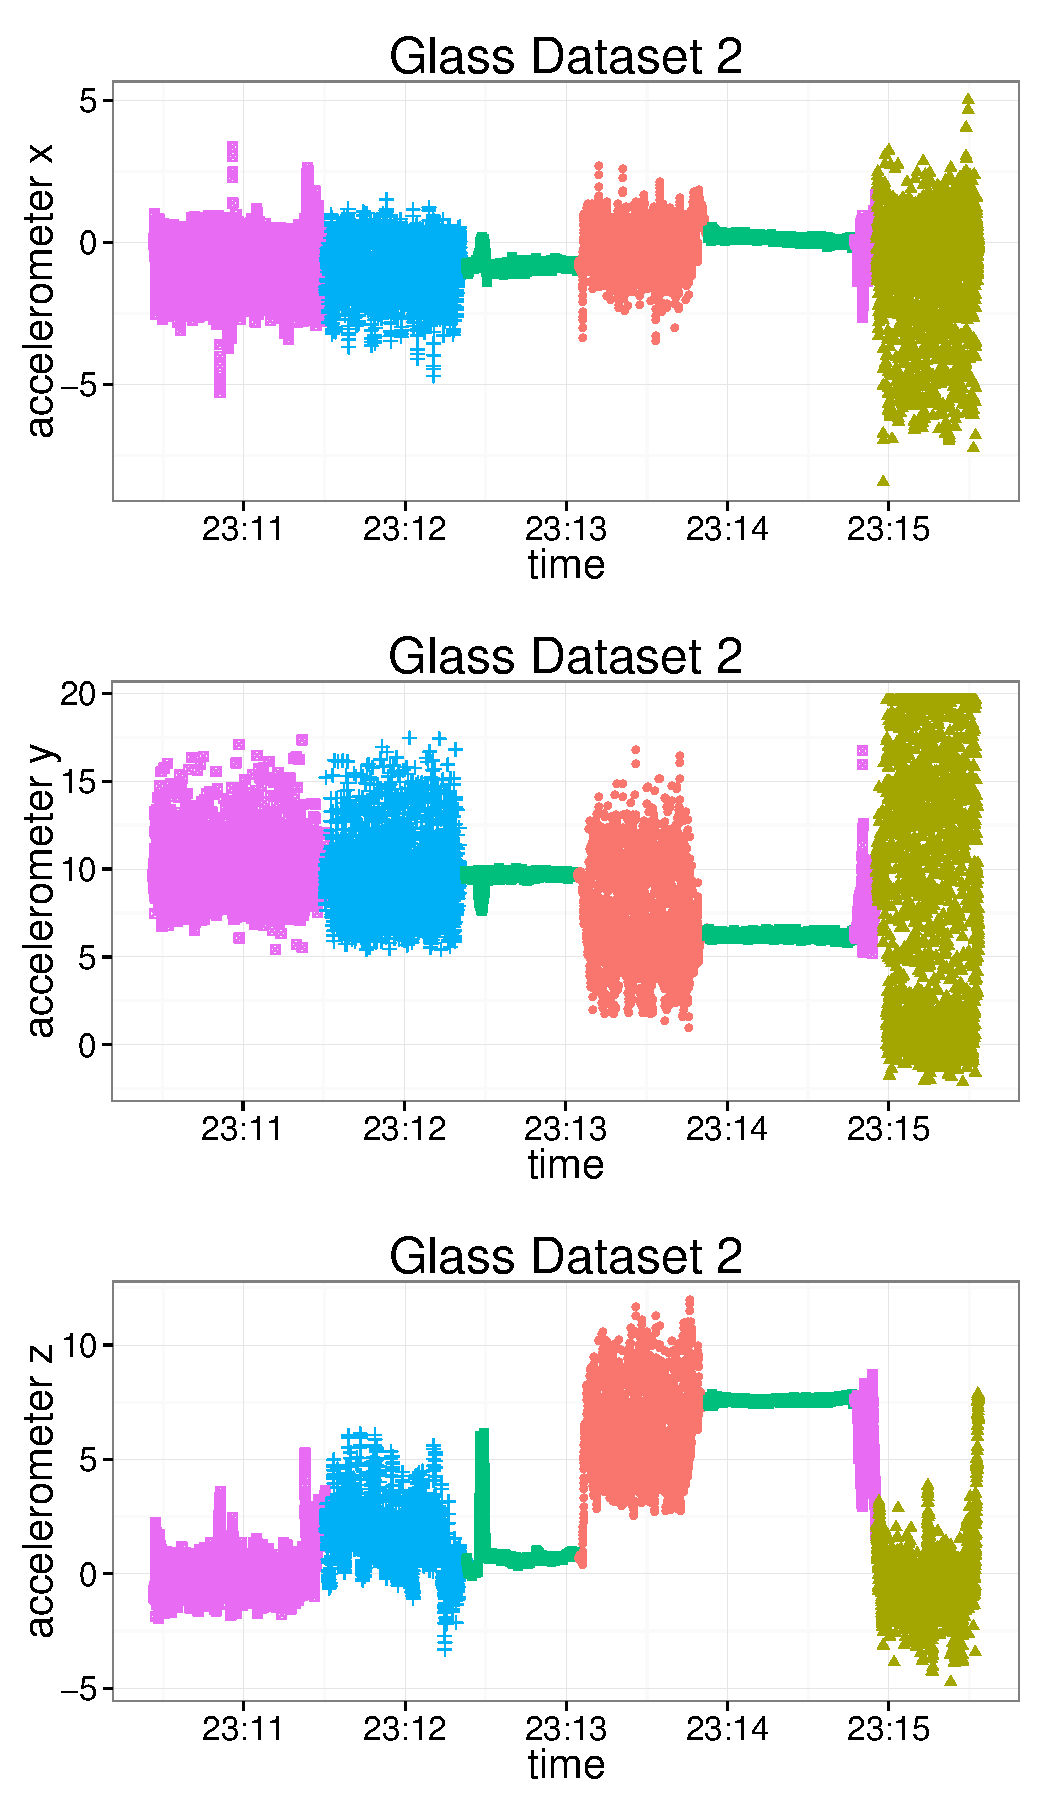
\includegraphics[width=0.3\textwidth]{figures/eda_soda2_glass.pdf}
  \includegraphics[width=0.3\textwidth]{figures/eda_soda2_phone.pdf}
  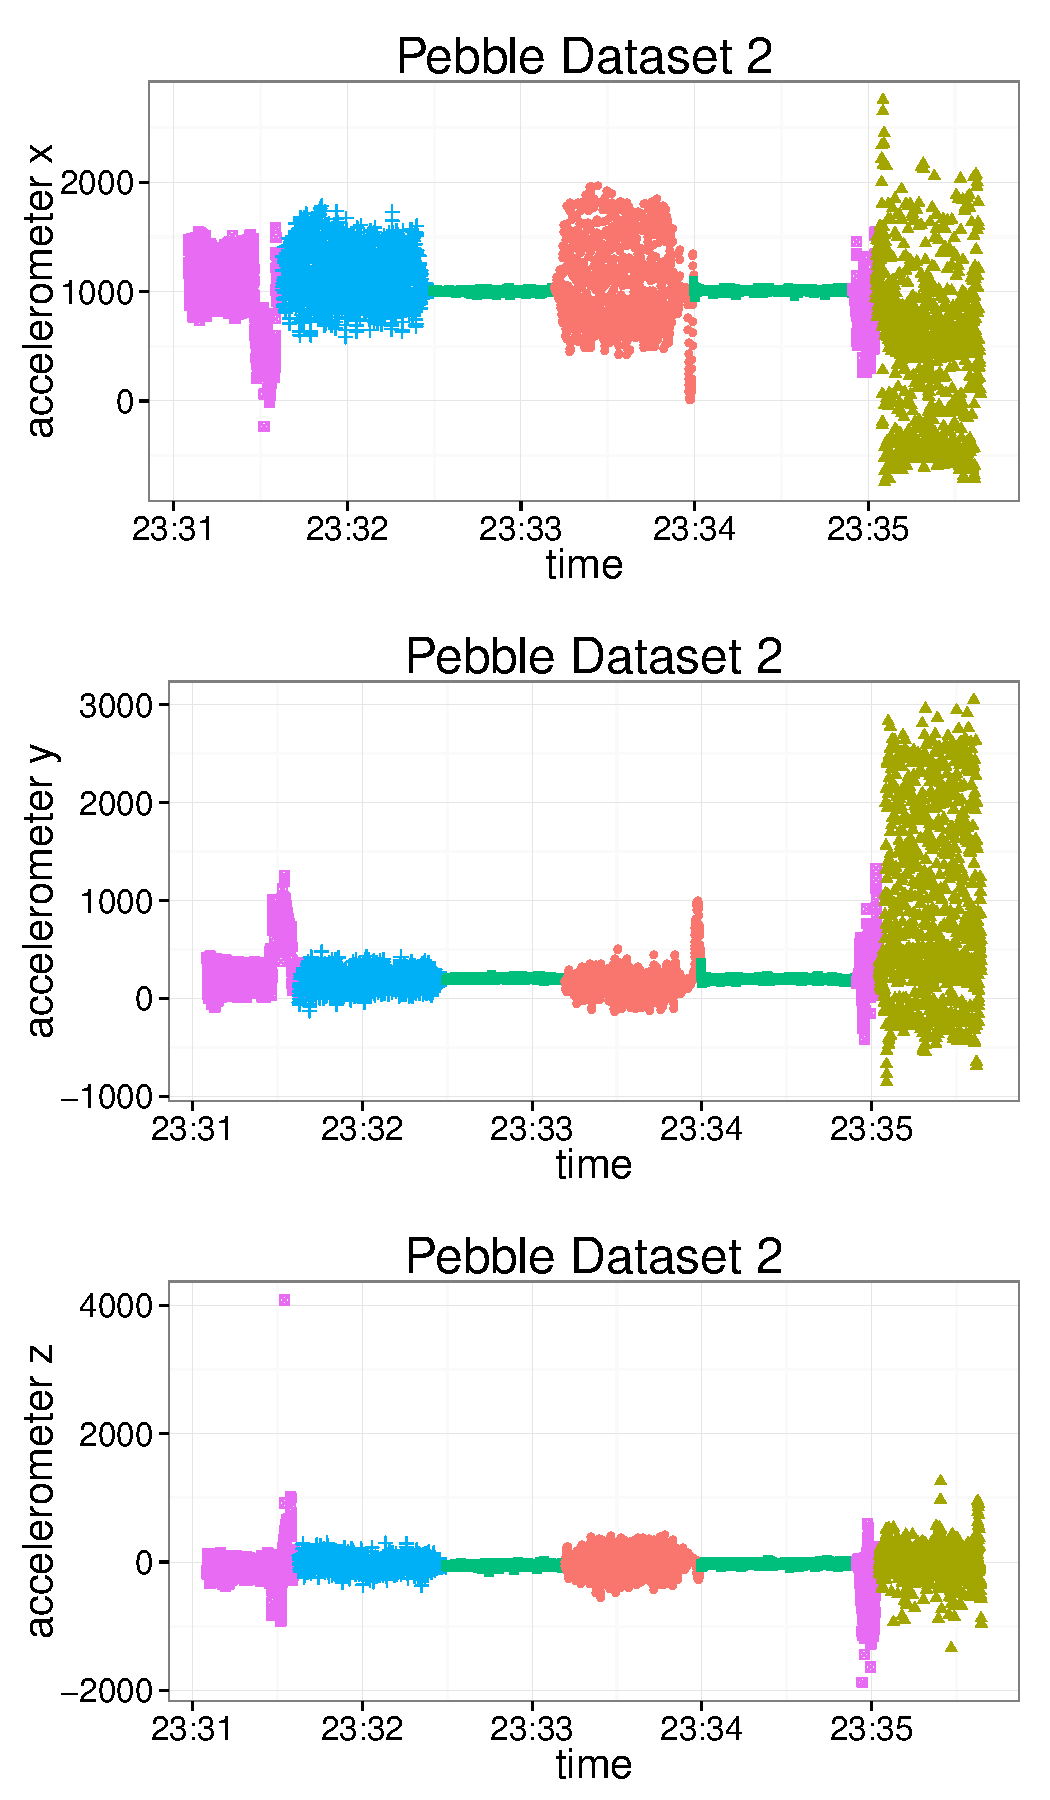
\includegraphics[width=0.3\textwidth]{figures/eda_soda2_pebble.pdf}
  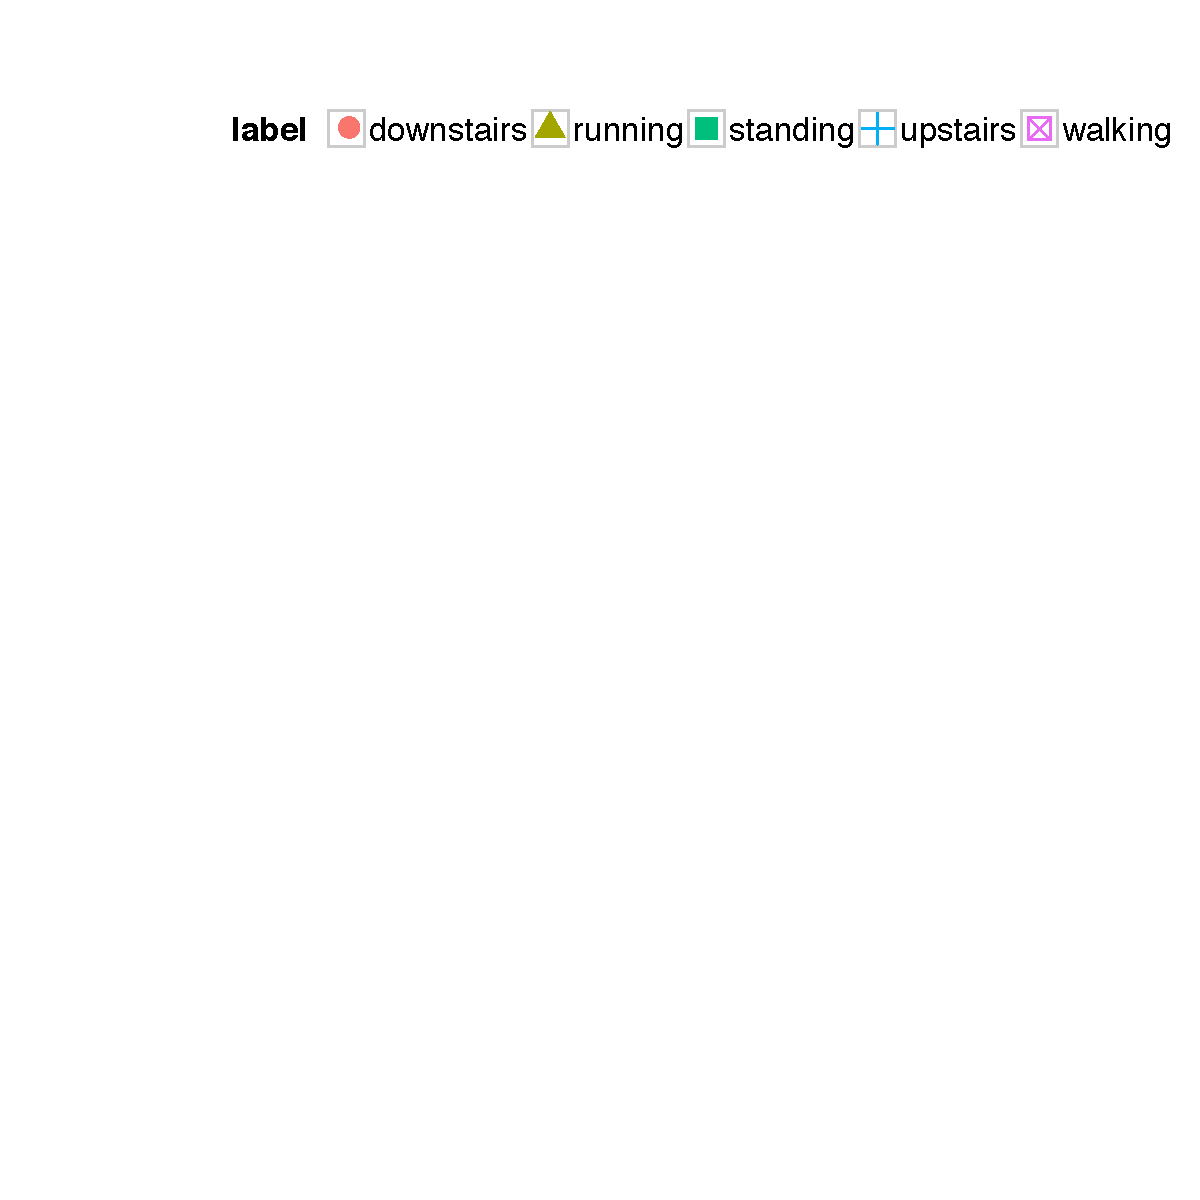
\includegraphics[width=0.5\textwidth]{figures/legend.pdf}
  \caption{The second raw data set visualization with groundtruth labeled.}
  \label{fig:soda2}
\end{figure*}

The empirical distribution for some selected features are shown in Figure~\ref{fig:features}. We choose proper family of distributions for our HMM model by inspecting these empirical distributions, for example, we have chosen $Gamma$ distribution for Entropy, and multivariate Gaussian for $\bar{x},\bar{y},\bar{z}$. 

\begin{figure}
  \centering
  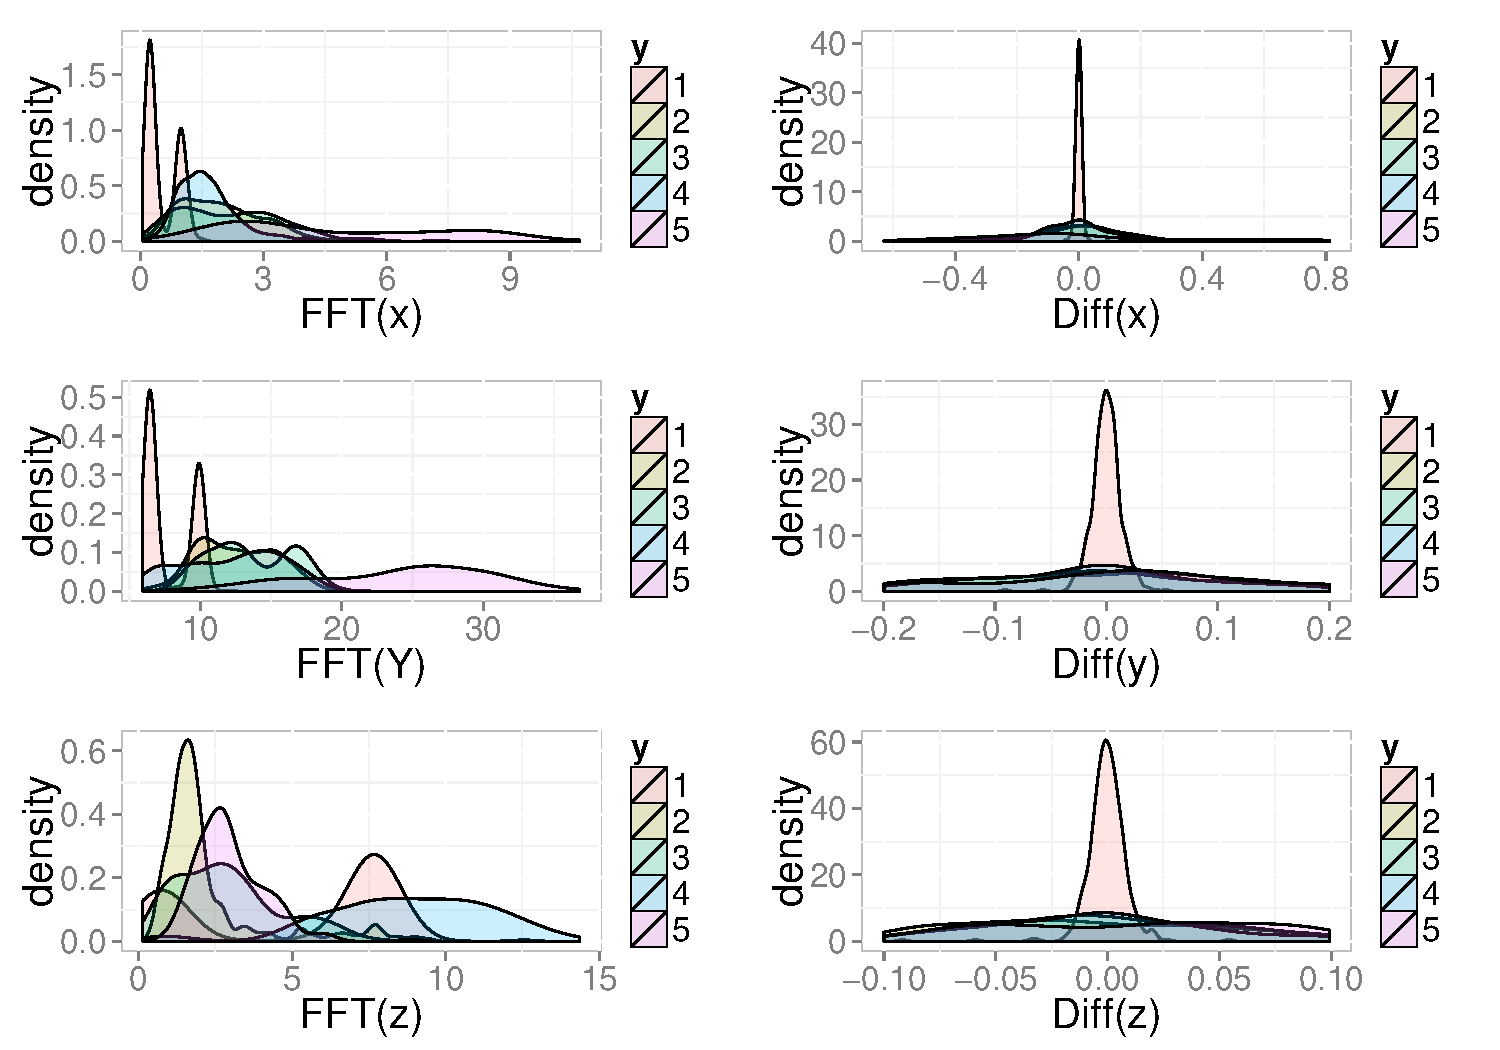
\includegraphics[width=0.5\textwidth]{figures/edafeature22.pdf}
  \caption{Empirical distribution for some selected features}
  \label{fig:features}
\end{figure}

In order to check the relation among features, we look at the pairwise scatter plot, and one example of these plots containing frequency domain feature is shown in Figure~\ref{fig:pairwise}. From this figure we can further justify the conditional dependence and independence of the features for HMM. For example, we use multivariate Gaussian instead of 
single Gaussian for $\bar{x},\bar{y},\bar{z}$, since they exhibit a strong correlation when conditioning on a specific activity.

\begin{figure}
  \centering
  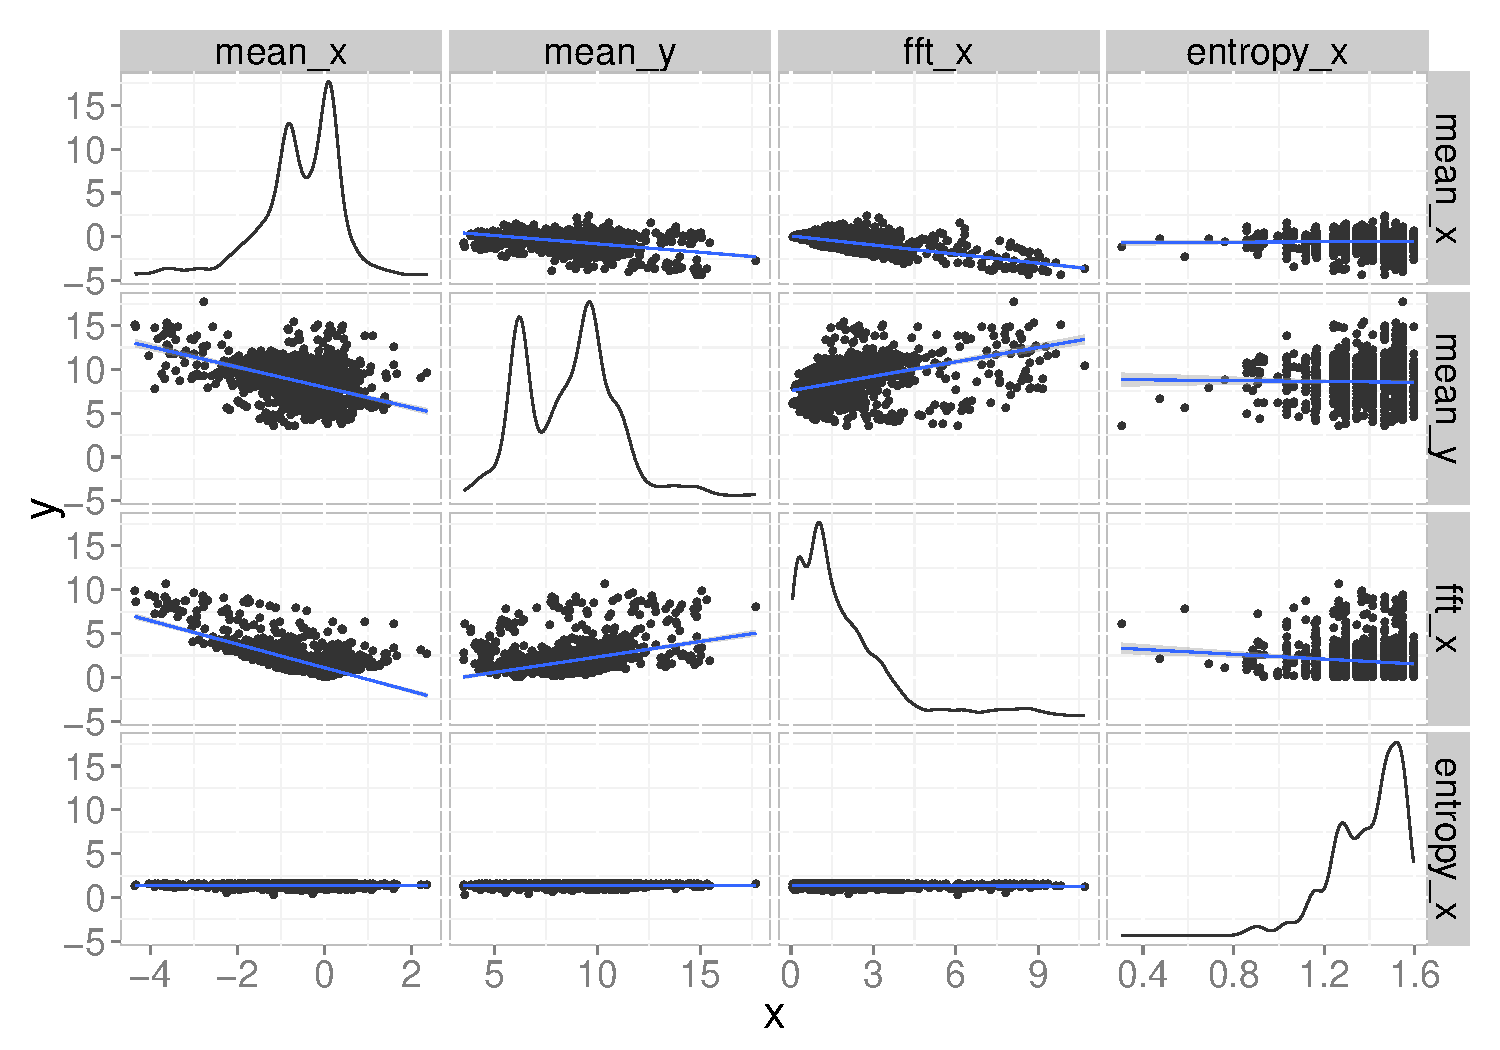
\includegraphics[width=0.48\textwidth]{figures/edafeature1.pdf}
  \caption{Pairwise scatter plot for some features}
  \label{fig:pairwise}
\end{figure}

\subsection{Classification Results}
Both model fitting and testing errors are summarized in terms of overall accuracy and cross error table to indicate the performance of activity recognition with three different devices and two different learning methods. Let's examine the results in a device order for easy comparison.

\subsubsection{Glass Results}
\label{sec:glassresult}

We summarize the results \textbf{with Multinomial Logistic Regression} in Table~\ref{tab:glassLR1}, \ref{tab:glassLR2} and \textbf{with HMM} in Table~\ref{tab:glassHMM1} and \ref{tab:glassHMM2}.

\begin{table}[!htb]
\begin{center}
\begin{tabular}{c|c}
      \hline
      Training Accuracy & Testing Accuracy\\
      \hline
      $0.9036635$ & $0.7469244$ \\
      \hline
\end{tabular}
\caption{Glass with LR: overall accuracy}
\label{tab:glassLR1}
\end{center}
\end{table}

\begin{table}[!htb]
\begin{center}
\begin{tabular}{c|c|c|c|c|c}
      \hline
      P/T& 1 & 2 &3 & 4 & 5 \\
      \hline
      1 &0.625&0.032&0.020&0.057&0.000\\
      2 &0.125&0.727&0.188&0.057&0.107\\
      3 &0.250&0.199&0.651&0.007&0.071\\
      4 &0.000&0.041&0.114&0.878&0.053\\
      5 & 0.000&0.000&0.026&0.000&0.767\\
      \hline
\end{tabular}
\caption{Glass with LR: Cross Error Table}
\label{tab:glassLR2}
\end{center}
\end{table}

\begin{table}[!htb]
\begin{center}
\begin{tabular}{c|c}
      \hline
      Training Accuracy & Testing Accuracy\\
      \hline
      $0.9599729$ & $0.7188049$ \\
      \hline
\end{tabular}
\caption{Glass with HMM: overall accuracy}
\label{tab:glassHMM1}
\end{center}
\end{table}
\begin{table}[h]
\begin{center}
\begin{tabular}{c|c|c|c|c|c}
      \hline
      P/T& 1 & 2 &3 & 4 & 5 \\
      \hline
      1 &0.400&0.057&0.006&0.029&0.000\\
      2 &0.066&0.692&0.240&0.067&0.155\\
      3 &0.133&0.211&0.629&0.022&0.017\\
      4 &0.400&0.033&0.110&0.880&0.068\\
      5 & 0.000&0.005&0.013&0.000&0.759\\
      \hline
\end{tabular}
\caption{Glass with HMM: Cross Error Table}
\label{tab:glassHMM2}
\end{center}
\end{table}

As expected, the testing error is much higher than training error for both Logistic Regression and HMM, while on testing set our system and algorithm still gives above 70\% accuracy. 

More interesting results can be revealed by looking at cross error table. Note that the number $\{1,2,...,5\}$ represent \{standing, walking, downstairs, upstairs, running\}. The rows of the table are ground truth and the columns are predicted value, thus the $\{i,j\}^{th}$ element of the table is interpreted as \textit{predicted value is $i$, while the true value should be $j$}. From this interpretation we see the diagonal terms in the table are actually accuracy in each class, and cross terms are different classification errors\footnote{We normalize the error in each class, however different classes may have different sample size.}.

We observe that in the case of using Google glass, the logistic regression method performs a little better than with HMM. Specifically, in both algorithms, Google glass distinguished very well the \textit{upstairs} state. Intuitively, this could be explained by the fact that when people are going upstairs, their head usually look up and maintains a distinct position, while in other states, people tend to move their head occasionally, which produce additional noise to Google glass measurement and harms the classification. This phenomena can also been seen especially from the fact that, for Google glass data with both algorithm, the standing state yields the most error.

Note also that we did not see improvement by incorporating transition (by using HMM), however, it does not exclude the benefit of transitional information. Actually, since our data set only measures a relatively short period, and the transitions of states are not statistically sufficient, we assume that for longer data with more complicated transitions, HMM method should show its advantages. 

\subsubsection{Phone Results} 
\label{subsec:phoneresult}

We summarize the results \textbf{with Multinomial Logistic Regression} in Table~\ref{tab:phoneLR1} and \ref{tab:phoneLR2}, and \textbf{with HMM} in Table~\ref{tab:phoneHMM1} and \ref{tab:phoneHMM2}.

\begin{table}[!htb]
\begin{center}
\begin{tabular}{c|c}
      \hline
      Training Accuracy & Testing Accuracy\\
      \hline
      $0.748297$ & $0.3341772$ \\
      \hline
\end{tabular}
\caption{Phone with LR: overall accuracy}
\label{tab:phoneLR1}
\end{center}
\end{table}

\begin{table}[!htb]
\begin{center}
\begin{tabular}{c|c|c|c|c|c}
      \hline
      P/T& 1 & 2 &3 & 4 & 5 \\
      \hline
      1 &0.593&0.125&0.071&0.017&0.000\\
      2 &0.196&0.125&0.313&0.366&0.318\\
      3 &0.125&0.000&0.306&0.241&0.181\\
      4 &0.129&0.125&0.282&0.294&0.272\\
      5 &0.062&0.625&0.026&0.080&0.227\\
      \hline
\end{tabular}
\caption{Phone with LR: Cross Error Table}
\label{tab:phoneLR2}
\end{center}
\end{table}

\begin{table}[!htb]
\begin{center}
\begin{tabular}{c|c}
      \hline
      Training Error & Testing Error\\
      \hline
      $0.9591281$ & $0.3578059$ \\
      \hline
\end{tabular}
\caption{Phone with HMM: overall accuracy}
\label{tab:phoneHMM1}
\end{center}
\end{table}
\begin{table}[!htb]
\begin{center}
\begin{tabular}{c|c|c|c|c|c}
      \hline
      P/T& 1 & 2 &3 & 4 & 5 \\
      \hline
      1 &1&0.014&0.064&0.006&0.000\\
      2 &0&0.542&0.303&0.635&0.158\\
      3 &0&0.136&0.335&0.155&0.123\\
      4 &0&0.188&0.271&0.162&0.341\\
      5 & 0&0.117&0.026&0.040&0.376\\
      \hline
\end{tabular}
\caption{Phone with HMM: Cross Error Table}
\label{tab:phoneHMM2}
\end{center}
\end{table}

We observe that both algorithm performed terribly on Phone data set. In effect, from previous part of EDA we already have a sense that Phone data set is more noisy and indistinguishable. The reason for that is simple: we put the Phone in the trousers pocket, and in all states except for standing, people's legs move periodically with a similar pattern. Hence we see that with Phone data set only the standing state is well classified, even with 1 accuracy with HMM, other states are mixed together and both classifiers only performs slightly better than a random guess. 

\subsubsection{Pebble Results}
\label{subsec:pebbleresult}

We summarize the results \textbf{with Multinomial Logistic Regression} in Table~\ref{tab:pebbleLR1} and \ref{tab:pebbleLR2}, and \textbf{with HMM} in Table~\ref{tab:pebbleHMM1} and \ref{tab:pebbleHMM2}.

\begin{table}[!htb]
\begin{center}
\begin{tabular}{c|c}
      \hline
      Training Accuracy & Testing Accuracy\\
      \hline
      $0.8658537$ & $0.6677966$ \\
      \hline
\end{tabular}
\caption{Pebble with LR: overall accuracy}
\label{tab:pebbleLR1}
\end{center}
\end{table}

\begin{table}[!htb]
\begin{center}
\begin{tabular}{c|c|c|c|c|c}
      \hline
      P/T& 1 & 2 &3 & 4 & 5 \\
      \hline
      1 &0.166&0.065&0.000&0.013&0.000\\
      2 &0.166&0.631&0.274&0.083&0.242\\
      3 &0.000&0.163&0.709&0.111&0.060\\
      4 &0.166&0.131&0.000&0.763&0.090\\
      5 &0.500&0.0082&0.016&0.027&0.606\\
      \hline
\end{tabular}
\caption{Pebble with LR: Cross Error Table}
\label{tab:pebbleLR2}
\end{center}
\end{table}

\begin{table}[!htb]
\begin{center}
\begin{tabular}{c|c}
      \hline
      Training Accuracy & Testing Accuracy\\
      \hline
      $0.9318902$ & $ 0.6237288$ \\
      \hline
\end{tabular}
\caption{Pebble with HMM: overall accuracy}
\label{tab:pebbleHMM1}
\end{center}
\end{table}
\begin{table}[!htb]
\begin{center}
\begin{tabular}{c|c|c|c|c|c}
      \hline
      P/T& 1 & 2 &3 & 4 & 5 \\
      \hline
      1 &0.5&0.063&0.000&0.019&0.000\\
      2 &0.0&0.618&0.370&0.182&0.080\\
      3 &0.5&0.218&0.555&0.183&0.000\\
      4 &0.0&0.081&0.074&0.596&0.000\\
      5 &0.0&0.018&0.000&0.019&0.920\\
      \hline
\end{tabular}
\caption{Pebble with HMM: Cross Error Table}
\label{tab:pebbleHMM2}
\end{center}
\end{table}

The results for Pebble data could be analyzed similarly. The performance of our classifier on this data set is in the middle of the performance on last two data sets. One interesting phenomenon is that the running state is very well classified, which could also be explained by intuition. When people are running, their forearm usually move with much higher frequency than in any other states. The classification of running versus other activities are relatively simple because in our feature selection procedure, we also include frequency domain features. 

%%% Local Variables: 
%%% mode: latex
%%% TeX-master: "main"
%%% End: 


\section{Related Work}
\label{sec:related-work}
\ben{This is just for adding the references. I have NOT read them well and summarized them well, so we need to change the texts.}
\yuxun{OK, I am doing it}

\cite{kwapisz2011activity} collected a large set of cell phone sensor data with labeled activities. A decision tree algorithm \footnote{J48 of Weka package} is mainly used for classification. However, according to our experiment and discussion, pocket phone accelerometer data is usually very noisy in that human leg movement is similar for some activities. We suggest that activity recognition can be greatly improved by considering various device measurements such as Google glass for head movement and Pebble watch for forearm movement.

\cite{srinivasan2012accurate,lee2011activity} focus on improving the recognition accuracy by building more complicated statistical models. For example, in \cite{srinivasan2012accurate}, a Two-Tier classifier is studied and in \cite{lee2011activity}, a Hierarchical Hidden Markov Model is considered. Nonetheless, these models suffers from complicated training step, and may not be tractable if more features from diverse devices are included. 

\cite{yan2012energy} discusses the energy consumption issues when using accelerometers in mobile devices for activity learning. They proposed a framework to adaptively choose sampling frequency when different activities are performed. This is important especially when measuring is conducted by consistently running application on cell phone, Google glass, or smart watches. The choice of sampling rate also constitutes our future works. 

 
%%% Local Variables: 
%%% mode: latex
%%% TeX-master: "main"
%%% End: 

\section{Conclusion}
\label{sec:conclusion}

To sum up, we have observed that measurements of different devices can help to distinguish different activities. As is mentioned above, this specialization comes from the fact that three devices are actually measuring the movement of different parts of human body. Therefore we propose that a combined sensoring system could greatly improve the classification performance of activity recognition. Major part of our future work will be devoted to this direction. 

%%% Local Variables: 
%%% mode: latex
%%% TeX-master: "main"
%%% End: 


\iftoggle{anonymous}{
% no acks in anonymous submission
}{
  \section{Acknowledgments}
  We deliver our sincere thanks to Prof.~Michael Jordan for his excellent teaching and explanation of a wide spectrum of statstical inference techniques. Kaifei Chen from SDB group has also helped us in developing the Android application using \texttt{BearLoc} project. Also Prof. Bj\"orn Hartmann is generous enough to lend us his Google Glass and Qualcomm Toq\footnote{Toq is not as friendly for programming as Pebble is. So we made the decision of using Pebble instead of Toq.} for the study. Moreover, many people are involved in the discussion of this project and how the study should be carried; without naming them one by one, we express our gratitude here.
}


% The following two commands are all you need in the
% initial runs of your .tex file to
% produce the bibliography for the citations in your paper.
\bibliographystyle{abbrv}
\bibliography{main}  % sigproc.bib is the name of the Bibliography in this case

% You must have a proper ".bib" file
%  and remember to run:
% latex bibtex latex latex
% to resolve all references
%
% ACM needs 'a single self-contained file'!
%
%APPENDICES are optional
%\balancecolumns
% \appendix
% %Appendix A
% \section{Headings in Appendices}
% The rules about hierarchical headings discussed above for
% the body of the article are different in the appendices.
% In the \textbf{appendix} environment, the command
% \textbf{section} is used to
% indicate the start of each Appendix, with alphabetic order
% designation (i.e. the first is A, the second B, etc.) and
% a title (if you include one).  So, if you need
% hierarchical structure
% \textit{within} an Appendix, start with \textbf{subsection} as the
% highest level. Here is an outline of the body of this
% document in Appendix-appropriate form:
% \subsection{Introduction}
% \subsection{The Body of the Paper}
% \subsubsection{Type Changes and  Special Characters}
% \subsubsection{Math Equations}
% \paragraph{Inline (In-text) Equations}
% \paragraph{Display Equations}
% \subsubsection{Citations}
% \subsubsection{Tables}
% \subsubsection{Figures}
% \subsubsection{Theorem-like Constructs}
% \subsubsection*{A Caveat for the \TeX\ Expert}
% \subsection{Conclusions}
% \subsection{Acknowledgments}
% \subsection{Additional Authors}
% This section is inserted by \LaTeX; you do not insert it.
% You just add the names and information in the
% \texttt{{\char'134}additionalauthors} command at the start
% of the document.

%\balancecolumns % GM June 2007
% That's all folks!
\end{document}

